%%%%%%%%%%%%%%
%% Run LaTeX on this file several times to get Table of Contents,
%% cross-references, and citations.

%% If you have font problems, you may edit the w-bookps.sty file
%% to customize the font names to match those on your system.

%% w-bksamp.tex. Current Version: Feb 16, 2012
%%%%%%%%%%%%%%%%%%%%%%%%%%%%%%%%%%%%%%%%%%%%%%%%%%%%%%%%%%%%%%%%
%
%  Sample file for
%  Wiley Book Style, Design No.: SD 001B, 7x10
%  Wiley Book Style, Design No.: SD 004B, 6x9
%
%
%  Prepared by Amy Hendrickson, TeXnology Inc.
%  http://www.texnology.com
%%%%%%%%%%%%%%%%%%%%%%%%%%%%%%%%%%%%%%%%%%%%%%%%%%%%%%%%%%%%%%%%

%%%%%%%%%%%%%
% 7x10
%\documentclass{wileySev}

% 6x9
\documentclass{wileySix}

\usepackage{graphicx}
\usepackage{listings}

\usepackage{color}
 
\definecolor{codegreen}{rgb}{0,0.6,0}
\definecolor{codegray}{rgb}{0.5,0.5,0.5}
\definecolor{codepurple}{rgb}{0.58,0,0.82}
\definecolor{backcolour}{rgb}{0.95,0.95,0.92}
 
\lstdefinestyle{mystyle}{
    backgroundcolor=\color{backcolour},   
    commentstyle=\color{codegreen},
    keywordstyle=\color{magenta},
    numberstyle=\tiny\color{codegray},
    stringstyle=\color{codepurple},
    basicstyle=\footnotesize,
    breakatwhitespace=false,         
    breaklines=true,                 
    captionpos=b,                    
    keepspaces=true,                 
    numbers=left,                    
    numbersep=5pt,                  
    showspaces=false,                
    showstringspaces=false,
    showtabs=false,                  
    tabsize=2,
    language=sh
}
 
\lstset{style=mystyle}

%%%%%%%
%% for times math: However, this package disables bold math (!)
%% \mathbf{x} will still work, but you will not have bold math
%% in section heads or chapter titles. If you don't use math
%% in those environments, mathptmx might be a good choice.

% \usepackage{mathptmx}

% For PostScript text
\usepackage{w-bookps}

%%%%%%%%%%%%%%%%%%%%%%%%%%%%%%%%%%%%%%%%%%%%%%%%%%%%%%%%%%%%%%%%
%% Other packages you might want to use:

% for chapter bibliography made with BibTeX
% \usepackage{chapterbib}

% for multiple indices
% \usepackage{multind}

% for answers to problems
% \usepackage{answers}

%%%%%%%%%%%%%%%%%%%%%%%%%%%%%%
%% Change options here if you want:
%%
%% How many levels of section head would you like numbered?
%% 0= no section numbers, 1= section, 2= subsection, 3= subsubsection
%%==>>
\setcounter{secnumdepth}{3}

%% How many levels of section head would you like to appear in the
%% Table of Contents?
%% 0= chapter titles, 1= section titles, 2= subsection titles, 
%% 3= subsubsection titles.
%%==>>
\setcounter{tocdepth}{2}

%% Cropmarks? good for final page makeup
%% \docropmarks

%%%%%%%%%%%%%%%%%%%%%%%%%%%%%%
%
% DRAFT
%
% Uncomment to get double spacing between lines, current date and time
% printed at bottom of page.
% \draft
% (If you want to keep tables from becoming double spaced also uncomment
% this):
% \renewcommand{\arraystretch}{0.6}
%%%%%%%%%%%%%%%%%%%%%%%%%%%%%%

%%%%%%% Demo of section head containing sample macro:
%% To get a macro to expand correctly in a section head, with upper and
%% lower case math, put the definition and set the box 
%% before \begin{document}, so that when it appears in the 
%% table of contents it will also work:

\newcommand{\VT}[1]{\ensuremath{{V_{T#1}}}}

%% use a box to expand the macro before we put it into the section head:

\newbox\sectsavebox
\setbox\sectsavebox=\hbox{\boldmath\VT{xyz}}

%%%%%%%%%%%%%%%%% End Demo


\begin{document}


\booktitle{PETUNJUK PENINGKATAN KOMPETENSI}
\subtitle{Dalam 24 Jam}

\authors{Rolly M. Awangga\\
\affil{Informatics Research Center}
%Floyd J. Fowler, Jr.\\
%\affil{University of New Mexico}
}

\offprintinfo{PETUNJUK PENINGKATAN KOMPETENSI , First Edition}{Rolly M. Awangga}

%% Can use \\ if title, and edition are too wide, ie,
%% \offprintinfo{Survey Methodology,\\ Second Edition}{Robert M. Groves}

%%%%%%%%%%%%%%%%%%%%%%%%%%%%%%
%% 
\halftitlepage

\titlepage


\begin{copyrightpage}{2019}
%Survey Methodology / Robert M. Groves . . . [et al.].
%\       p. cm.---(Wiley series in survey methodology)
%\    ``Wiley-Interscience."
%\    Includes bibliographical references and index.
%\    ISBN 0-471-48348-6 (pbk.)
%\    1. Surveys---Methodology.  2. Social 
%\  sciences---Research---Statistical methods.  I. Groves, Robert M.  II. %
%Series.\\
%
%HA31.2.S873 2007
%001.4'33---dc22                                             2004044064
\end{copyrightpage}

\dedication{`Jika Kamu tidak dapat menahan lelahnya belajar, 
Maka kamu harus sanggup menahan perihnya Kebodohan.'
~Imam Syafi'i~}

\begin{contributors}
\name{Rolly Maulana Awangga,} Informatics Research Center., Politeknik Pos Indonesia, Bandung,
Indonesia



\end{contributors}

\contentsinbrief
\tableofcontents
\listoffigures
\listoftables
\lstlistoflistings


\begin{foreword}
Sepatah kata dari Kaprodi, Kabag Kemahasiswaan dan Mahasiswa
\end{foreword}

\begin{preface}
Buku ini diciptakan bagi yang awam dengan git sekalipun.

\prefaceauthor{R. M. Awangga}
\where{Bandung, Jawa Barat\\
Februari, 2019}
\end{preface}


\begin{acknowledgments}
Terima kasih atas semua masukan dari para mahasiswa agar bisa membuat buku ini 
lebih baik dan lebih mudah dimengerti.

Terima kasih ini juga ditujukan khusus untuk team IRC yang 
telah fokus untuk belajar dan memahami bagaimana buku ini mendampingi proses 
Intership.
\authorinitials{R. M. A.}
\end{acknowledgments}

\begin{acronyms}
\acro{ACGIH}{American Conference of Governmental Industrial Hygienists}
\acro{AEC}{Atomic Energy Commission}
\acro{OSHA}{Occupational Health and Safety Commission}
\acro{SAMA}{Scientific Apparatus Makers Association}
\end{acronyms}

\begin{glossary}
\term{git}Merupakan manajemen sumber kode yang dibuat oleh linus torvald.

\term{bash}Merupakan bahasa sistem operasi berbasiskan *NIX.

\term{linux}Sistem operasi berbasis sumber kode terbuka yang dibuat oleh Linus Torvald
\end{glossary}

\begin{symbols}
\term{A}Amplitude

\term{\hbox{\&}}Propositional logic symbol 

\term{a}Filter Coefficient

\bigskip

\term{\mathcal{B}}Number of Beats
\end{symbols}

\begin{introduction}

%% optional, but if you want to list author:

\introauthor{Rolly Maulana Awangga, S.T., M.T.}
{Informatics Research Center\\
Bandung, Jawa Barat, Indonesia}

Pada era disruptif  \index{disruptif}\index{disruptif!modern} 
saat ini. git merupakan sebuah kebutuhan dalam sebuah organisasi pengembangan perangkat lunak.
Buku ini diharapkan bisa menjadi penghantar para programmer, analis, IT Operation dan Project Manajer.
Dalam melakukan implementasi git pada diri dan organisasinya.

Rumusnya cuman sebagai contoh aja biar keren\cite{awangga2018sampeu}.

\begin{equation}
ABC {\cal DEF} \alpha\beta\Gamma\Delta\sum^{abc}_{def}
\end{equation}

\end{introduction}

%%%%%%%%%%%%%%%%%%Isi Buku_

\chapter{Judul Bagian Pertama}
\section{Perintah Navigasi}
Perintah navigasi direktori


\chapter{Tugas Pokok}
\textbf{Penilaian tugas pokok dilakukan setiap satu minggu sekali dengan mengakumulasikan jumlah pekerjaan per-parameter selama 1 minggu.}

\section{Dedikasi}

Menurut KBBI, Dedikasi bisa diartikan sebagai suatu pengorbanan tenaga, pikiran, dan waktu demi keberhasilan suatu usaha atau tujuan yang mulia. Dalam kata lain dedikasi juga bisa diartikan sebagai pengabdian. Pengabdian atau dedikasi yang bisa dilakukan mahasiswa D4 Teknik Informatika yaitu dengan melakukan pembuatan ataupun pembaharuan modul ajar di \textbf{\textit{https://github.com/bukuinformatika}}.

Adapun parameter penilaian dedikasi dapat dilihat pada tabel \ref{tab:nilaidedikasi}.

\begin{table}[H]
\caption{Penilaian Dedikasi}
\centering
\begin{tabular}{|c|c|c|c|}
\hline
\textbf{No.}&\textbf{Label}&\textbf{Nilai}&\textbf{Keterangan}\\
\hline
1.&TINGGI&3&Full commit selama 5 hari kerja\\
\hline
2.&SEDANG&2&Commit selama 4 hari kerja\\
\hline
3.&RENDAH&1&Commit kurang dari 4 hari kerja\\
\hline
\end{tabular}
\label{tab:nilaidedikasi}
\end{table}

\section{Produktifitas}
Produktivitas mengandung arti sebagai perbandingan antara hasil yang dicapai (output) dengan keseluruhan sumber daya yang digunakan (input). Dengan kata lain bahwa produktivitas memliliki dua dimensi. Dimensi pertama adalah efektivitas yang mengarah kepada pencapaian target berkaitan dengan kuaitas, kuantitas dan waktu. Yang kedua yaitu efisiensi yang berkaitan dengan upaya membandingkan input dengan realisasi penggunaannya atau bagaimana pekerjaan tersebut dilaksanakan.

Adapun parameter penilaian produktifitas dapat dilihat pada tabel \ref{tab:nilaiproduktifitas}.

\begin{table}[H]
\caption{Penilaian Produktifitas}
\centering
\begin{tabular}{|c|c|c|c|}
\hline
\textbf{No.}&\textbf{Label}&\textbf{Nilai}&\textbf{Keterangan}\\
\hline
1.&TINGGI&3&Mengerjakan 5 pekerjaan harian\\
\hline
2.&SEDANG&2&Mengerjakan 4 pekerjaan harian\\
\hline
3.&RENDAH&1&Mengerjakan kurang dari 4 pekerjaan harian\\
\hline
\end{tabular}
\label{tab:nilaiproduktifitas}
\end{table}

\section{Integritas}
Integritas merupakan salah satu atribut terpenting/kunci yang harus dimiliki seorang pemimpin. Integritas adalah suatu konsep berkaitan dengan konsistensi dalam tindakan-tindakan, nilai-nilai, metode-metode, ukuran-ukuran, prinsip-prinsip, ekspektasi-ekspektasi dan berbagai hal yang dihasilkan.

Adapun parameter penilaian integritas dapat dilihat pada tabel \ref{tab:nilaiintegritas}.

\begin{table}[H]
\caption{Penilaian Integritas}
\centering
\begin{tabular}{|c|c|c|c|}
\hline
\textbf{No.}&\textbf{Label}&\textbf{Nilai}&\textbf{Keterangan}\\
\hline
1.&TINGGI&3&Tidak ada penolakan pull request\\
\hline
2.&SEDANG&2&Ada 1 penolakan pull request\\
\hline
3.&RENDAH&1&Ada lebih dari 1 penolakan pull request\\
\hline
\end{tabular}
\label{tab:nilaiintegritas}
\end{table}

Catatan:
\begin{itemize}
\item Selesaikan konflik terlebih dahulu, untuk menghindari penolakan saat pull request.
\end{itemize}

\section{Disiplin}
Disiplin merupakan perasaan taat dan patuh terhadap nilai-nilai yang dipercaya merupakan tanggung jawabnya. Dengan kata lain disiplin adalah patuh terhadap peraturan atau tunduk pada pengawasan dan pengendalian. Sedangkan pendisiplinan adalah usaha usaha untuk menanamkan nilai ataupun pemaksaan agar subjek memiliki kemampuan untuk menaati sebuah peraturan.

Adapun parameter penilaian disiplin dapat dilihat pada tabel \ref{tab:nilaidisiplin}.

\begin{table}[H]
\caption{Penilaian Disiplin}
\centering
\begin{tabular}{|c|c|c|c|}
\hline
\textbf{No.}&\textbf{Label}&\textbf{Nilai}&\textbf{Keterangan}\\
\hline
1.&TINGGI&3&Datang pulang sesuai jadwal selama 5 hari kerja\\
\hline
2.&SEDANG&2&Ada 1 hari terlambat ataupun tidak masuk\\
\hline
3.&RENDAH&1&Ada lebih dari 1 hari terlambat ataupun tidak masuk\\
\hline
\end{tabular}
\label{tab:nilaidisiplin}
\end{table}

\section{Loyalitas}
Loyalitas yang dimaksud yaitu usaha untuk menjaga kenyamanan dan keamanan lingkungan kerja. Contoh dari loyalitas diantaranya:
\begin{enumerate}
\item Menjaga area kerja tetap bersih dan bebas dari debu;
\item Menjaga kerapihan dan kenyaman area kerja;
\item Memperbaiki perangkat kerja yang rusak, dll.
\end{enumerate}
Adapun parameter penilaian loyalitas dapat dilihat pada tabel \ref{tab:nilailoyalitas}.

\begin{table}[H]
\caption{Penilaian Loyalitas}
\centering
\begin{tabular}{|c|c|c|c|}
\hline
\textbf{No.}&\textbf{Label}&\textbf{Nilai}&\textbf{Keterangan}\\
\hline
1.&TINGGI&3&Area kerja bersih tanpa debu selama 5 hari kerja\\
\hline
2.&SEDANG&2&Ada 1 hari area kerja tidak bersih\\
\hline
3.&RENDAH&1&Ada lebih dari 1 hari area kerja tidak bersih\\
\hline
\end{tabular}
\label{tab:nilailoyalitas}
\end{table}

\section{Kreatif dan Inisiatif}

Adapun parameter penilaian kreatif dan inisiatif dapat dilihat pada tabel \ref{tab:nilaikreatifinisiatif}.

\begin{table}[H]
\caption{Penilaian Kreatif dan Inisiatif}
\centering
\begin{tabular}{|c|c|c|c|}
\hline
\textbf{No.}&\textbf{Label}&\textbf{Nilai}&\textbf{Keterangan}\\
\hline
1.&TINGGI&3&Menjadi tentor dengan jumlah peserta minimal 10 orang\\
\hline
2.&SEDANG&2&Menjadi tentor dengan jumlah peserta minimal 5 orang\\
\hline
3.&RENDAH&1&Menjadi tentor dengan jumlah peserta kurang dari 5 orang\\
\hline
\end{tabular}
\label{tab:nilaikreatifinisiatif}
\end{table}

Catatan:
\begin{enumerate}
\item Kegiatan ini dilaksanakan minimal 1 kali selama Internship II berlangsung, dengan catatan target poin terpenuhi.
\item Kegiatan yang dilaksanakan merupakan kegiatan berbayar ataupun bersponsor.
\item Target poin yang dicapai minimal 3.
\item Jika poin tidak memenuhi target, maka silahkan untuk mengadakan kegiatan lagi sampai jumlah poin minimal terpenuhi.
\end{enumerate} 

\chapter{Standar Latex dan Git}
\section{Standar latex dan git}

\begin{enumerate}
\item sebelum melakukan langkah pull reques alangkah baik anda mempelajari materi git di github.com/bukuinformatika/git (buka file git.pdf)
\item buka github awangga/ppji (cari ppji.pdf untuk melihat penulisan standar latex)
\item buka github.com/bukuinformatika/keleketek (untuk mempelajari materi dasar latex)
\end{enumerate}

 langkah-langkah Pull request menggunakan GIT BASH:
\begin{enumerate}
\item git pull origin master
\item git pull upstream master
\item git push origin master
\item edit file yang akan di pull reques
\item setelah anda selesai edit/tambah file comflile dulu di main.tex agar anda tahu pekerjaan yang anda lakukan tidak bermasalah.
\item git status
\item git add 'namafile\_sesui\_setatus'
\item git status 
\item commit -m 'melakukan apa yang anda edit'
\item git status
\item git pull upstream master
\item git push origin master
\end{enumerate}

Buka repositori anda untuk new pull request:
\begin{enumerate}
\item Klik New Pull request
\item Klik tombol hijau seperti pada gambar lihat tanda yang diberi kotak warna merah \ref{labelgambar1} 
		\begin{figure}[htbp]
		\centering
		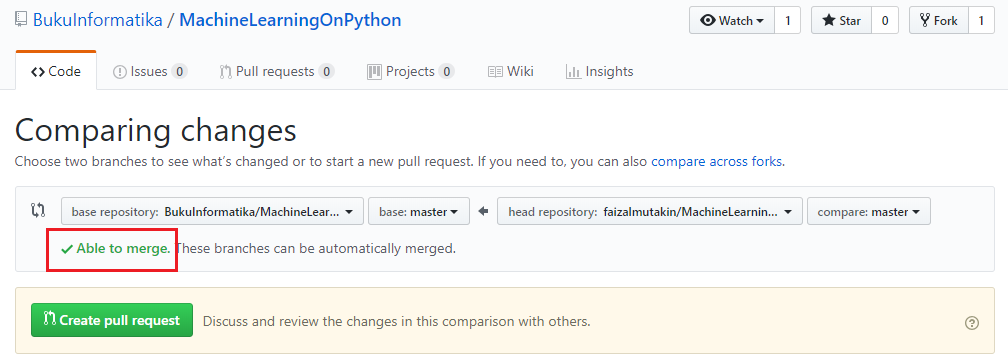
\includegraphics[width=1\textwidth]{figures/1.PNG}
		\caption{Gambar new pull requesh}
		\label{labelgambar1}
		\end{figure}	 
\end{enumerate}



\bibliographystyle{IEEEtran} 
%\def\bibfont{\normalsize}
\bibliography{references}


%%%%%%%%%%%%%%%
%%  The default LaTeX Index
%%  Don't need to add any commands before \begin{document}
\printindex

%%%% Making an index
%% 
%% 1. Make index entries, don't leave any spaces so that they
%% will be sorted correctly.
%% 
%% \index{term}
%% \index{term!subterm}
%% \index{term!subterm!subsubterm}
%% 
%% 2. Run LaTeX several times to produce <filename>.idx
%% 
%% 3. On command line, type  makeindx <filename> which
%% will produce <filename>.ind 
%% 
%% 4. Type \printindex to make the index appear in your book.
%% 
%% 5. If you would like to edit <filename>.ind 
%% you may do so. See docs.pdf for more information.
%% 
%%%%%%%%%%%%%%%%%%%%%%%%%%%%%%

%%%%%%%%%%%%%% Making Multiple Indices %%%%%%%%%%%%%%%%
%% 1. 
%% \usepackage{multind}
%% \makeindex{book}
%% \makeindex{authors}
%% \begin{document}
%% 
%% 2.
%% % add index terms to your book, ie,
%% \index{book}{A term to go to the topic index}
%% \index{authors}{Put this author in the author index}
%% 
%% \index{book}{Cows}
%% \index{book}{Cows!Jersey}
%% \index{book}{Cows!Jersey!Brown}
%% 
%% \index{author}{Douglas Adams}
%% \index{author}{Boethius}
%% \index{author}{Mark Twain}
%% 
%% 3. On command line type 
%% makeindex topic 
%% makeindex authors
%% 
%% 4.
%% this is a Wiley command to make the indices print:
%% \multiprintindex{book}{Topic index}
%% \multiprintindex{authors}{Author index}

\end{document}

